\begin{enumerate}

  \item \emph{Compute the one-step matrix.} \smallskip \newline
  In the one-step matrix, if the energy flows from a prey to the predator, then the effect of the prey on the predator is the reciprocal of the indegree of the predator

            \begin{equation}
              a_{1,ij}=\frac{A_{ij}}{D_j}
            \end{equation}

  \item \emph{Compute the n-step matrices.} \smallskip \newline
  In the higher steps matrices, a node influences another node at a higher trophic level by summing the effects of every path that connects the two nodes. The effect of every path is the multiplication of the inverse of the outdegree of every node along the path. For a visual explanation see Figure \ref{fig:TI}. It can be calculated as follows

            \begin{equation}
              A\left(n\right)=A_{\left(1\right)}^n
            \end{equation}

  \item \emph{Calculate topological importance} \smallskip \newline
  The topological importance of a node i ($TI_i$) can be calculated through the following formula

            \begin{equation}
              TI_i=\frac{\sum\limits^N_{m=1}\sum\limits^n_{j=1}a_{m,ji}}{N}
            \end{equation}

  \noindent where $N$ is the total number of steps considered, $m$ is the step number,  $n$ is the total number of nodes, and $a_{m,ji}$ is the effect of species $i$ on species $j$ at $m$ number of steps.

            \begin{figure}[htbp]%{\textwidth}
              \centering
              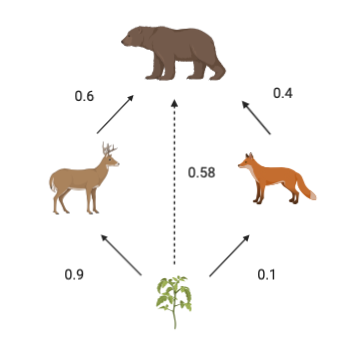
\includegraphics[width=1.0\linewidth]{TI_example.png}
              \caption{Topological importance (TI) of a species on another. The plant and the bear are not connected, so there is no direct effect from the plant to the bear. However, indirect effects reach the bear from the plant through two paths and the final effect is the sum of these effects. The first one is through the deer and the second is through the fox. The strength of these paths is the product of the direct effects composing the path. The first path has an effect on the bear that is 0.9*0.6=0.54, the second one has an effect on the bear that is 0.1*0.4=0.04. Summing the effects through these two 2-step paths connecting the plant with the bear, we get the 2-step effect of the plant on the bear: 0.54+0.04=0.58. Figure created with BioRender.com.} \label{fig:TI}
            \end{figure}

\end{enumerate}
